Les ordinateurs sont des outils très puissants, pour peu qu'on arrive à leur communiquer ce qu'on aimerait obtenir. On entend souvent dire qu'un ordinateur ne comprend qu'un langage très basique : le langage binaire, une suite de 0 et de 1. Du point de vue des microprocesseurs, on peut voir ça ainsi : soit le courant passe, soit il ne passe pas. En combinant ces deux états d'une manière bien précise, on peut effectuer des calculs.

Cependant, écrire un quelconque programme directement en binaire, c'est quasiment mission impossible, même pour un programme très basique. Il faut passer par une étape de traduction, et c'est ici que ça devient intéressant! L'idée générale est d'écrire du code dans un langage de programmation, et de le transformer en langage machine/binaire.

Il y a deux manières de traduire du code.
\begin{itemize}
    \item \emph{La compilation :} On convertit immédiatement le code en langage machine. L'avantage, c'est que l'ordinateur comprend directement. Par contre, il faudra recommencer cette étape pour chaque système d'exploitation différents (Windows, macOS, Linux, ...).
    \item \emph{L'interprétation :} on va ici passer par un intermédiaire : \textit{l'interpréteur}. C'est un programme qui lit et traduit le code en temps réel. C'est un processus plus lent, mais qui offre un grand avantage : on ne doit plus faire plusieurs versions pour chaque système d'exploitation, puisque c'est l'interpréteur qui se charge de la traduction! On dit d'un tel langage qu'il est \textit{multi-plateformes}.
\end{itemize}

%%% Au cours, on peut donner un exemple : compilation = traduire un texte en chinois et en arabe. Interprétation = le donner à un mec qui sait parler chinois et arabe. On doit pas traduire nous-même mais ça prend plus de temps.

Il existe une autre manière de classer les langages de programmation. Au plus ils ressemblent à du langage machine, au plus ils sont \textit{bas niveau}. Au contraire, au plus un langage de programmation se rapproche du langage humain, au plus il est \textit{haut-niveau}.

Le Python est un langage interprété, et haut-niveau, ce qui en fait un excellent choix pour débuter en programmation : on peut l'exécuter aisément sur de nombreux systèmes d'exploitation, et le code est assez lisible. Mais il ne faut pas s'y tromper : ce n'est pas parce qu'il est haut-niveau qu'il n'est pas puissant, bien au contraire!

\begin{figure}[t]
	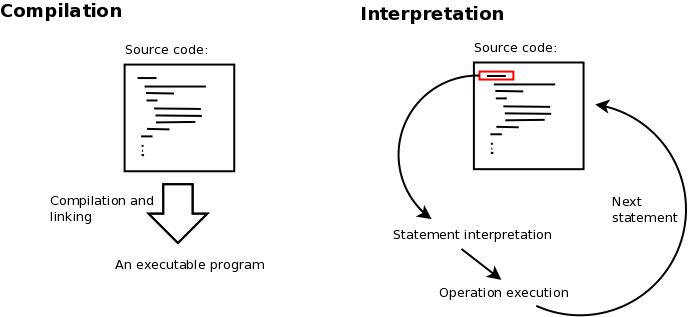
\includegraphics[width=\textwidth]{inter.png}
	\caption{Langage compilé vs langage interprété}
\end{figure}
